% IEEEAerospace2012.cls requires the following packages: times, rawfonts, oldfont, geometry
\documentclass[5p]{elsarticle}  % only supports two-column, letterpaper format

% The next line gives some packages you may find useful for your paper--these are not required though.
%\usepackage[]{graphicx,float,latexsym,amssymb,amsfonts,amsmath,amstext,times,psfig}
% NOTE: The .cls file is now compatible with amsmath!!!


\usepackage[english]{babel}
\usepackage{afterpage}
%\usepackage{multicol}
\usepackage{array}
\usepackage{fancyhdr}
%\usepackage{palatino}
%\usepackage[tight,nice]{units}
\usepackage{float}
\usepackage{times}
\usepackage{booktabs}
%\usepackage[pdftex]{graphicx}
\usepackage{url}
%\usepackage{eurosym}
\usepackage{mathtools}
\usepackage{amsmath,amssymb,amsfonts}
\usepackage{hyperref}
\usepackage[acronym,nomain]{glossaries}

%\usepackage{subfig}
%\usepackage{caption}
%\usepackage{subcaption}
\usepackage{multirow}
%\usepackage[bottom=3cm,left=2.75cm,right=2.75cm,head=0.75cm]{geometry} 
\usepackage{gensymb}
\usepackage{xcolor}			
%\usepackage{colortbl}
\usepackage{lastpage}			
%\usepackage{cite}			
%\usepackage{listings}
%\usepackage[absolute]{textpos}
%\usepackage{rotating}	
%\usepackage{background}
%\usepackage{lscape} 
% \usepackage{helvet} 
%\usepackage{tgpagella}
%\usepackage{todonotes}
%\usepackage{longtable}
%\usepackage{epstopdf}


%---- All images can be stored in a separate directory  ----%
\graphicspath{{fig/}}

% Assign bibliography style (which typically works for Acta Astronautica later 
\bibliographystyle{elsarticle-num}

% -------This is an example on how to use acronyms----------- %
% This section can be deleted  
\newacronym{solve}{SOLVE}{Satellites Observing Lakes and Vegetation Environments}
\newacronym{uav}{UAV}{Unmanned Aerial Vehicle} 
\newacronym{hap}{HAP}{High Altitude Platform} 
\newacronym{eSpace}{eSpace}{EPFL Space Engineering Center}
\newacronym{APHYS}{APHYS}{Physics of Aquatic Systems Laboratory (EPFL)}
\newacronym{EPSL}{EPSL}{Earth and Planetary Science Laboratory (EPFL)}
\newacronym{MRS}{MRS}{Multimodal Remote Sensing Laboratory (University of Zurich)} 
\newacronym{RSL}{RSL}{Remote Ssensing Laboratory (University of Zurich)} 

\newacronym{MDR}{MDR}{Mission Definition Review} 
\newacronym{PRR}{PRR}{Preliminary Requirements Review} 
\newacronym{PDR}{PDR}{Preliminary Design Review} 
\newacronym{CDR}{CDR}{Critical Design Review} 
\newacronym{GSD}{GSD}{Ground Sample Distance}
\newacronym{SNR}{SNR}{Signal to Noise Ratio}

\newacronym{TRL}{TRL}{Technology Readiness Level}
\newacronym{ADCS}{ADCS}{Attitude Determination and Control Subsystem} 
\newacronym{COM}{COM}{Communication subsystem}
\newacronym{EPS}{EPS}{Energy and Power System}
\newacronym{CDMS}{CDMS}{Control and Data Management subsystem}
\newacronym{UAV}{UAV}{Unmanned Aerial Vehicle}
\newacronym{HAP}{HAP}{High Altitutde Platform}
\newacronym{FPS}{FPS}{Frames Per Second}
\newacronym{CDF}{CDF}{Concurrent Design Facility}

\newacronym{HSI}{HSI}{HyperSpectral Imager}
\newacronym{GPU}{GPU}{Graphics Processing Unit}
\newacronym{COTS}{COTS}{Commercial Off-The-Shelf}

\newcommand{\ignore}[1]{}  % {} empty inside = %% comment

\makeglossaries

\pagestyle{fancy}
\chead{\textit{ {\small 74th International Astronautical Congress (IAC), Baku, Azerbaijan, 02-07 October 2023. \\
Copyright ©2017 by the International Astronautical Federation (IAF). All rights reserved.} }
}
\lhead{}
\rhead{}

\begin{document}
	
\begin{frontmatter}


  % CHange title to your paper here, follow the format 
	\title{IAC-17-B5.1.1 \\ \sc{Business Case Development for Precision Agriculture Applications using UAV and Space Borne Platforms.}}
	\tnotetext[mytitlenote]{IAC-17-B5.1.1,x36950}
	
	%% Group authors per affiliation:
	\author{}
	\address{Propulsion and Space Research Center, Technology Innovation Institute, Masdar City, Abu Dhabi, United Arab Emirates}
	\ead{xxx.xxx@tii.ae}
	% \fntext[myfootnote]{Since 1880.}
	
	%% or include affiliations in footnotes:
	%\author[mymainaddress,mysecondaryaddress]{Elsevier Inc}
	%\ead[url]{www.elsevier.com}
	
	%\author[mysecondaryaddress]{Global Customer Service\corref{mycorrespondingauthor}}
	%\cortext[mycorrespondingauthor]{Corresponding author}
	%\ead{support@elsevier.com}
	
	%\address[mymainaddress]{1600 John F Kennedy Boulevard, Philadelphia}
	%\address[mysecondaryaddress]{360 Park Avenue South, New York}
	
\begin{abstract}
     %ADD the ABSTRACT 

\end{abstract}
	
\begin{keyword}
  
\end{keyword}
\end{frontmatter}
	

%%%% IMPORTANT: Use the correct copyright information--IEEE, Crown, or U.S. government. %%%%%
%\thanks{Satellites Observing Lakes and Vegetation Environments (SOLVE)}
%\thanks{\footnotesize 978-1-5090-1613-6/17/$31.00$ \copyright2017 IEEE}              % This creates the copyright info that is the correct 2016 data.
%\thanks{{U.S. Government work not protected by U.S. copyright}}         % Use this copyright notice only if you are employed by the U.S. Government.
%\thanks{{978-1-5090-1613-6/17/$\$31.00$ \copyright2017 Crown}}          % Use this copyright notice only if you are employed by a crown government (e.g., Canada, UK, Australia).
%\thanks{{978-1-5090-1613-6/17/$\$310.00$ \copyright2017 European Union}}    % Use this copyright notice is you are employed by the European Union.


%\maketitle

%\thispagestyle{plain}
%\pagestyle{plain}


%\tableofcontents
%\printglossary

%%%%%%%%%%%%%%%%%%%%%%%%%%%%%%%%%%%%%%
\section{Introduction}
%%%%%%%%%%%%%%%%%%%%%%%%%%%%%%%%%%%%%%
\label{sec:introduction}

%......... here 1 page of motivation why we're doing this, summary text from the other text 
\section{Objectives of the Paper} 
\label{sec:mission_objectives} 


\section{State of the Art}
\label{sec:market}


% Example how to include a figure 
\begin{figure}[h]
  \centering
  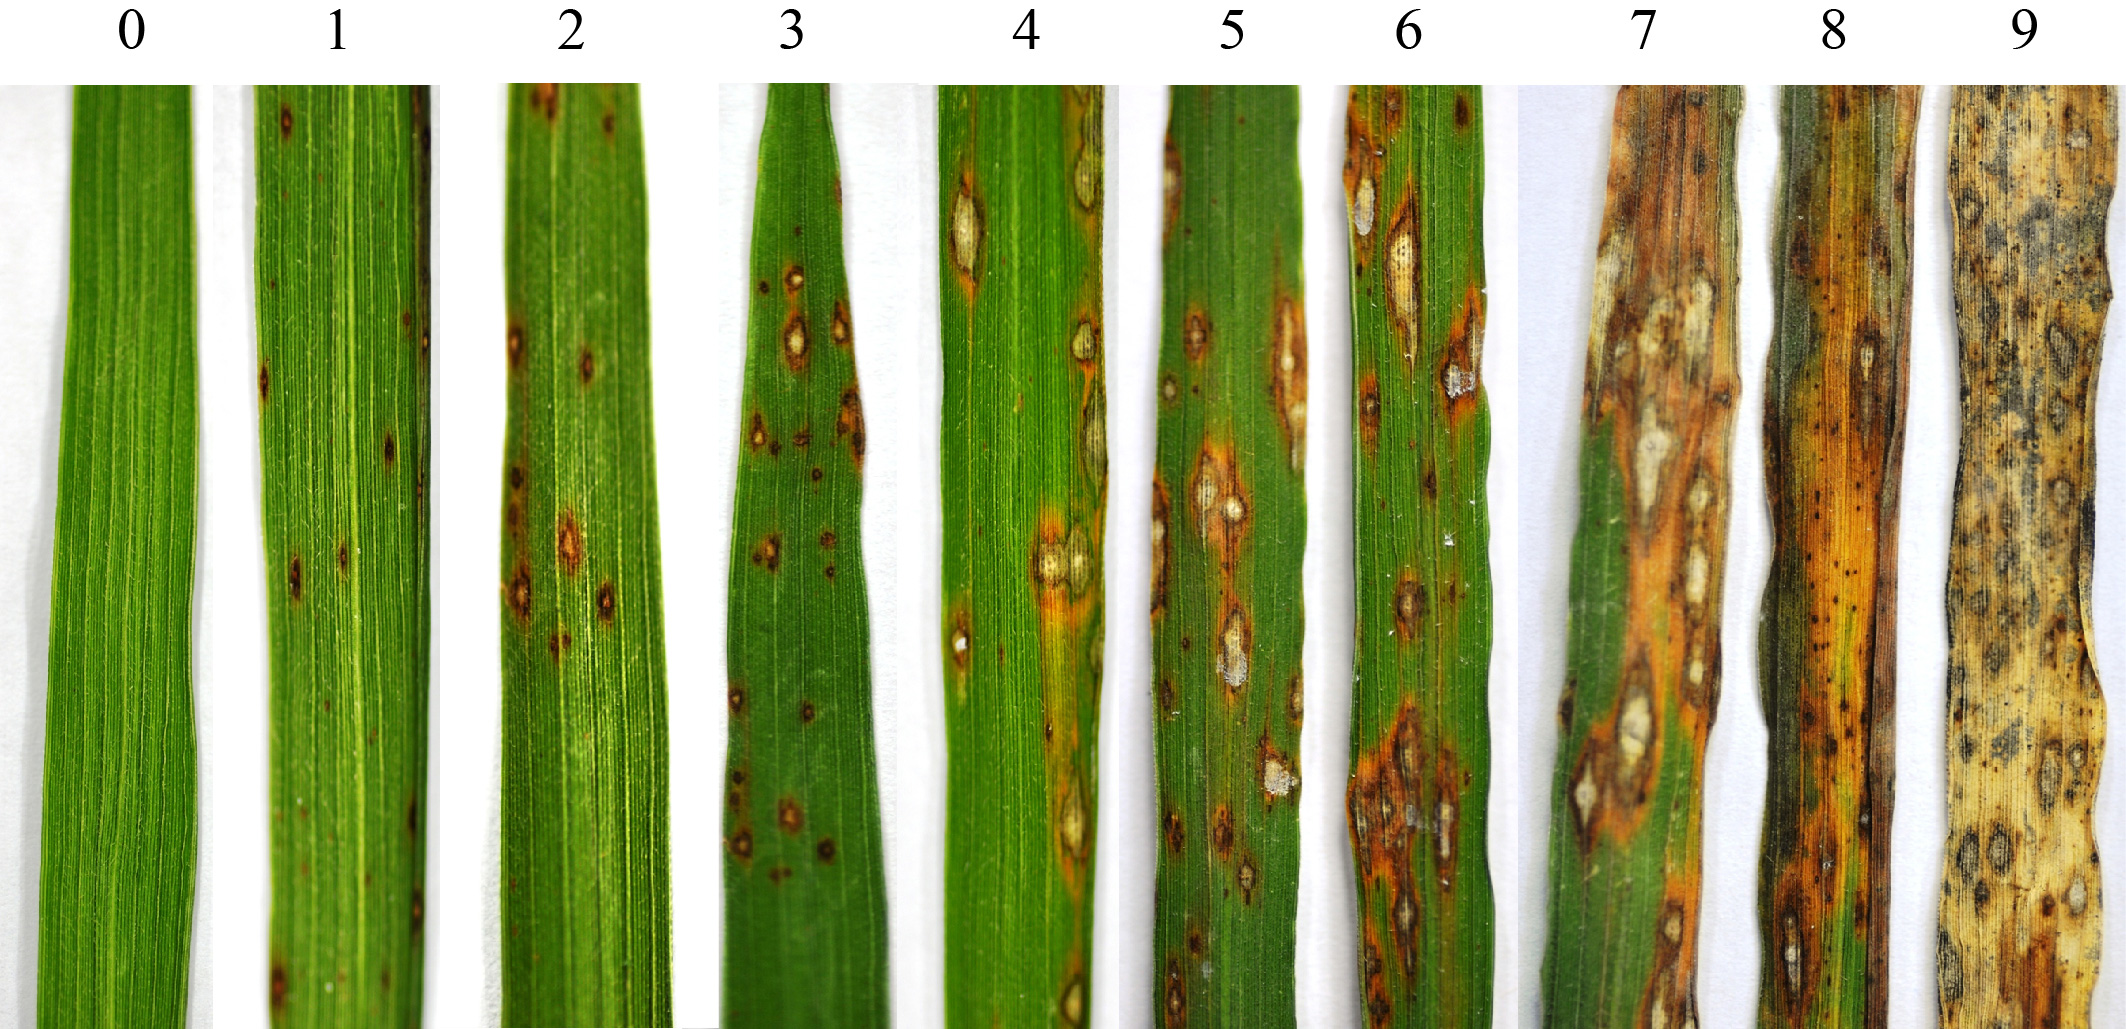
\includegraphics[width=0.42 \textwidth]{figure/rice_blast.jpeg}
  \caption{Scoring scale for leaf blast susceptibility, from \cite{ethz16}}
  \label{fig:blast}
\end{figure}
  
\section{Technology Assessment}
  \label{Tech_part}

This investigation is summarized in Table \ref{tab:tech_char}.

%%%%% Example how to make a table 

\renewcommand{\arraystretch}{1.5}
\begin{table*}[htbp]
  \centering
  \begin{tabular}{|c|>{\centering}m{3cm}|c|>{\centering}m{3.5cm}|>{\centering}m{2.5cm}|c|}  
    \hline
       \textbf{Crop}&\textbf{Disease}&\textbf{Spatial res.}&\textbf{Spectral bands}&\textbf{Tracking period [days]}&\textbf{Yield loss [\%]}\\
       % \hhline{|=|=|=|=|=|=|}
       \hline
        \multirow{2}{*}{Rice} &Bacterial Blight \cite{yang10}&n/a &757-1039 nm&1-3&up to 70\\   
        \cline{2-6}
        &Rice Blast \cite{kob01} &1 m &combination of 530-570 \&
650-700 nm&1-2&10-30\\
        \hline
                \multirow{2}{*}{Corn} &Common Smut&\multicolumn{2}{c|}{no literature} &1-5&5-30\\   
        \cline{2-6}
        &NCLB&\multicolumn{2}{c|}{no literature} &1-4&30\\
        \hline
                \multirow{2}{*}{Wheat} &FHB \cite{bau11}& n/a & 665-675 \& 550-560 nm&1-2&20-50\\   
        \cline{2-6}
        &Yellow Rust \cite{huang07} &1 m &400-850 nm&1-5&5-30\\
      	\hline
        Weed &Ambrosia \cite{Goss14}&\textless1.8 m &450-900 nm&1-3&9-25, up to 60\\
        \hline
  \end{tabular}      
  \caption{Observational characteristics of the different diseases in the visible spectrum, suitable for hyperspectral technologies}
  \label{tab:tech_char}
\end{table*}


\subsection{Summary}

The array of systems, presented in Table \ref{tab:cpblts} gives a whole range of remote sensing possibilities. Generally, the higher the system flies, the higher is its coverage capabilities while the resolution is inversely proportional. 

	\begin{table*}[t]
     \centering
%\begin{tabular}{|>{\centering}m{2cm}|>{\centering}m{1.6cm}|>{\centering}m{1.8cm}|>{\centering}m{1.4cm}|>{\centering}m{1.6cm}|>{\centering}m{2cm}|c|}  
\begin{tabular}{|>{\centering}m{2cm}|>{\centering}m{1.4cm}|>{\centering}m{1.4cm}|>{\centering}m{1.4cm}|>{\centering}m{1.4cm}|>{\centering}m{1.6cm}|p{1.2cm}|p{4.2cm}|}
\cline{1-8}
\textbf{Carrier}&\textbf{Spatial res.}&\textbf{Auto- nomy}&\textbf{Cruise speed}&\textbf{Swath width}&\textbf{Coverage} [ha/h]&\textbf{Revisit time}&\textbf{Comments}\\
\hline
\hline
%\hhline{|=|=|=|=|=|=|=|=|}
Near-ground drone &$>$1 cm&\textless 2 h &90 km/h&100 m &900 &Daily&Constraint by weather,  range and regulations\\   
\cline{1-8}
%\hline
Stratospheric drone &$>$10 cm& Days/ weeks &100 km/h&1 km &10k &Daily&Constraints due to cloud coverage \& regulations\\   
\cline{1-8}
 Small satellite constellation & $>$10 m&Years&8 km/s&100 km &300M &2 days&High up front cost, spatial resolution\\   
\cline{1-8}     
 Large satellite &$>$5 m&Years&7 km/s&200 km &600M &6 days&Operated by agency, data cost might be high, spatial res.\\   
\cline{1-8} 
\end{tabular}
\caption{Indicative capabilities of different systems for agricultural remote sensing}
\label{tab:cpblts}
        \end{table*}


\section{Discussion} 

\section{Conclusions} 

%%%%%%%%%%%%%%%%%%%%%%%%%%%%%%%%%%%%%%%%%%%%%%%%%%%%%%%%%%%%%%%%%%%%%%%%%%%%%%%%%%%%%%%%%%%%%%%%%%%%%% 
\section*{Acknowledgments}

\section*{References}

%%%%%%%%%%%%%%%%%%%%%%%%%%%%%%%%%%%%%%%%%%%%%%%%%%%%%%%%%%%%%%%%%%%%%%%%%%%%%%%%%%%%%%%%%%%%%%%%%%%%%%
%\bibliographystyle{IEEEtran}
\bibliography{biblio_science.bib}% Reference documents (e.g. ECSS)


%\bibliography{IEEEabr,MyBibFile}


%%%%%%%%%%%%%%%%%%%%%%%%%%%%%%%%%%%%%%%%%%%%%%%%%%%%%%%%%%%%%%%%%%%%%%%%%%%%%%%%%%%%%%%%%%%%%%%%%%%%%%

\end{document}
